\let\negmedspace\undefined
\let\negthickspace\undefined
\documentclass[journal]{IEEEtran}

\usepackage[a5paper, margin=10mm, onecolumn]{geometry}
%\usepackage{lmodern} % Uncomment if needed for pdflatex
\usepackage{tfrupee} % Include tfrupee package

\setlength{\headheight}{1cm} % Set the height of the header box
\setlength{\headsep}{0mm}     % Set the distance between the header box and the top of the text

\usepackage{gvv-book}
\usepackage{gvv}
\usepackage{cite}
\usepackage{amsmath,amssymb,amsfonts,amsthm}
\usepackage{algorithmic}
\usepackage{graphicx}
\usepackage{textcomp}
\usepackage{txfonts}
\usepackage{listings}
\usepackage{enumitem}
\usepackage{mathtools}
\usepackage{gensymb}
\usepackage{comment}
\usepackage[breaklinks=true]{hyperref}
\usepackage{tkz-euclide} 
\usepackage{inputenc}                                        
\usepackage{color}                                            
\usepackage{array}                                            
\usepackage{longtable}                                       
\usepackage{calc}                                             
\usepackage{multirow}                                         
\usepackage{hhline}                                           
\usepackage{ifthen}                                           
\usepackage{lscape}
\usepackage{tikz}
\usepackage{circuitikz}
\usepackage{standalone} % For including external TikZ files
\usepackage{longtable}

\begin{document}

\bibliographystyle{IEEEtran}
\vspace{3cm}

\title{Clock}
\author{EE24BTECH11066 - YERRA AKHILESH}
\maketitle

\renewcommand{\thefigure}{\theenumi}
\renewcommand{\thetable}{\theenumi}
\setlength{\intextsep}{10pt} % Space between text and floats

\numberwithin{equation}{enumi}
\numberwithin{figure}{enumi}
\renewcommand{\thetable}{\theenumi}


\section{Seven-Segment Display Connections}

The digital clock consists of six seven-segment displays, which are connected in a multiplexed configuration to minimize the number of control pins. The connections are made as follows:

\subsection{Segment Interconnections}
Each segment (a to g) of all six displays is wired together to ensure proper synchronization. The connection pattern is:

\begin{itemize}
    \item The ‘a’ pin of the first seven-segment display (from the left) is connected to the ‘a’ pin of the second display.
    \item The ‘a’ pin of the second display is connected to the ‘a’ pin of the third.
    \item This pattern continues for all six displays.
\end{itemize}

Similarly, repeat this process for the \textbf{b, c, d, e, f, and g} pins.
This setup ensures that all corresponding segments across all displays light up together when controlled.

\subsection{Resistor Placement}

\begin{itemize}
    \item Each seven-segment display has a resistor connected to its middle pin (common cathode).
    \item The other end of each resistor is connected to the digital pins on the Arduino from pin 11V down to pin 6V.
    \item This setup limits current flow, preventing excessive power draw and ensuring proper display brightness.
\end{itemize}

\section{7447 BCD to 7-Segment Decoder Connections}

The 7447 decoder is responsible for translating binary-coded decimal (BCD) signals into segment control signals for the display. The connections are as follows:

\subsection{7447 to Seven-Segment Display}

\begin{itemize}
    \item The ‘a’ output (pin 13) of the 7447 is connected to the ‘a’ segment pin of the last (6th) seven-segment display.
    \item The same pattern follows for all segment outputs:
    \begin{itemize}
        \item b’ (pin 12) $\rightarrow$ ‘b’ segment of the 6th display.
        \item c’ (pin 11) $\rightarrow$ ‘c’ segment of the 6th display.
        \item d’ (pin 10) $\rightarrow$ ‘d’ segment of the 6th display.
        \item e’ (pin 9) $\rightarrow$ ‘e’ segment of the 6th display.
        \item f’ (pin 15) $\rightarrow$ ‘f’ segment of the 6th display.
        \item g’ (pin 14) $\rightarrow$ ‘g’ segment of the 6th display.\\
    \end{itemize}
\end{itemize}

Refer the below 7447 circuit diagram to make the connections easier,

\begin{figure}[h!]
   \centering
   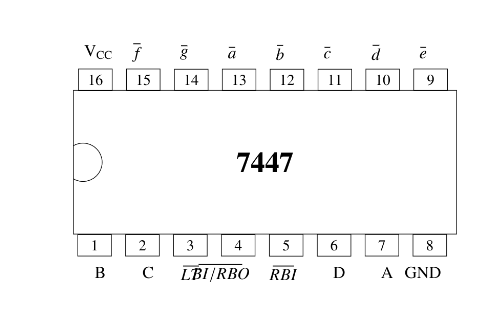
\includegraphics[width=0.65\columnwidth]{figs/7447.png}
   \label{stemplot}
\end{figure}
\subsection{Power and Ground Connections}

\begin{itemize}
    \item Vcc (pin 16) of the 7447 is connected to the 5V rail.
    \item GND (pin 8) is connected to the ground rail (GND) of the Arduino.
\end{itemize}

\subsection{BCD Input Connections (Arduino to 7447)}

The BCD input pins of the 7447 receive signals from the Arduino digital pins as follows:

\begin{itemize}
    \item A (pin 7) $\rightarrow$ Connected to 2V pin on the Arduino.
    \item B (pin 1) $\rightarrow$ Connected to 3V pin on the Arduino.
    \item C (pin 2) $\rightarrow$ Connected to 4V pin on the Arduino.
    \item D (pin 6) $\rightarrow$ Connected to 5V pin on the Arduino.
\end{itemize}

This configuration allows the Arduino to send binary values to the 7447, which then converts them into appropriate signals for displaying digits.


\section{Key Features regarding the code part}  
\vspace{0.2cm}  

\subsection{Three Operating Modes}  
\vspace{0.3cm}  
\begin{itemize}  
    \item \textbf{Clock Mode} – Keeps track of real-time hours, minutes, and seconds, updating automatically every second.  
    \item \textbf{Timer Mode} – Functions as a countdown timer where users can set hours and minutes.  
    \item \textbf{Stopwatch Mode} – Allows users to measure elapsed time with start and stop functionality.  
\end{itemize}  
\vspace{0.2cm}  

\subsection{User Controls for Easy Operation}  
\vspace{0.3cm}  
\begin{itemize}  
    \item \textbf{Mode Selection:} A button on \textbf{PB0} switches between Clock, Timer, and Stopwatch modes.  
    \item \textbf{Time Adjustment:} Buttons on \textbf{PD6} and \textbf{PD7} allow users to manually increase hours and minutes in Clock and Timer modes. 
    \item \textbf{Start/Stop Control:} A button on \textbf{PB1} starts and stops the Stopwatch or Timer.  
\end{itemize}  
\vspace{0.5cm}  

\subsection{Smart Display Multiplexing for Efficiency}  
\vspace{0.3cm}  
\begin{itemize}  
    \item A \textbf{BCD to 7-segment decoder (7447)} is used to simplify digit control.  
    \item \textbf{Fast multiplexing} ensures all six digits are updated rapidly, preventing display lag.  
    \item The display refresh rate is optimized to \textbf{avoid flickering}, making it clear and easy to read.  
\end{itemize}  
\vspace{0.5cm}  

\subsection{Accurate Timekeeping with Timer Interrupts}  
\vspace{0.3cm}  
\begin{itemize}  
    \item \textbf{Timer1 runs in CTC mode}, generating an exact \textbf{1-second interval} for stable time tracking.  
    \item The \textbf{Interrupt Service Routine (ISR)} automatically updates the clock, timer, and stopwatch, eliminating the need for delays.  
    \item This approach \textbf{reduces CPU load} and ensures smooth performance without interfering with other tasks.  
\end{itemize}  

\begin{figure}[h!]
   \centering
   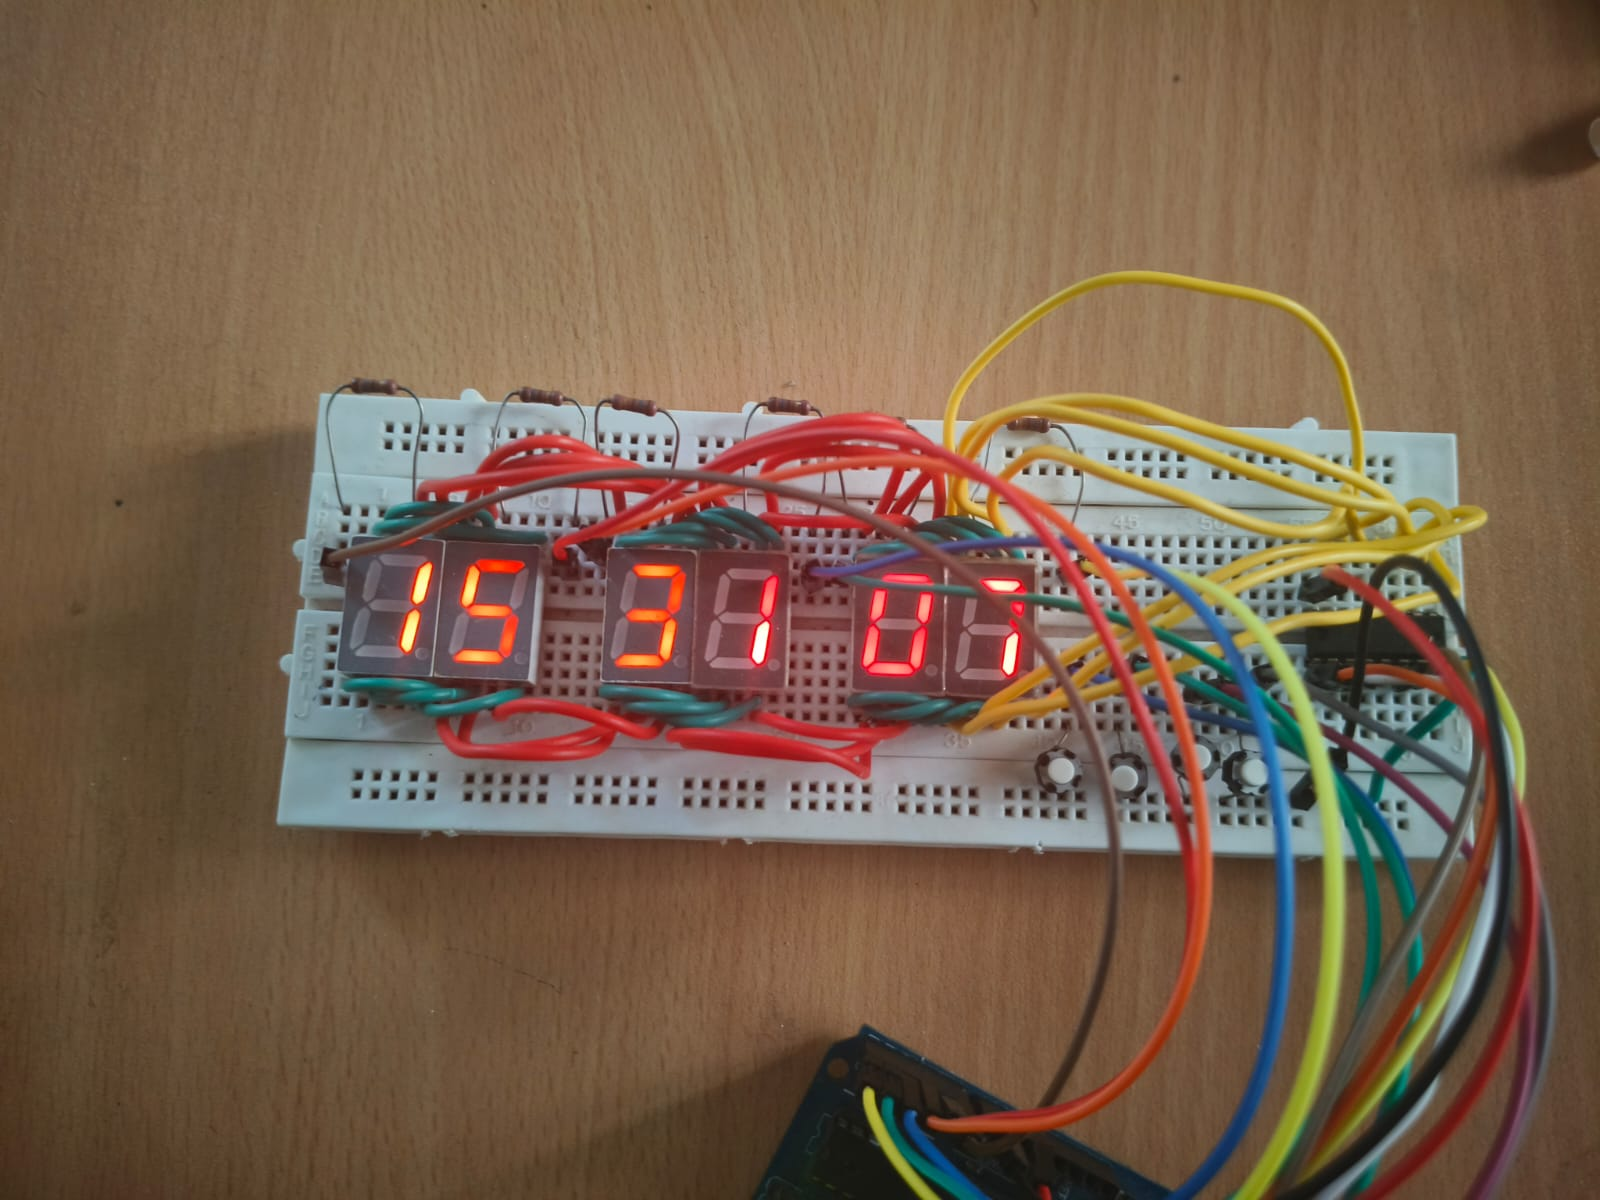
\includegraphics[width=0.50\columnwidth]{figs/timer.jpeg}
   \label{stemplot}
\end{figure}
This is the connections part to show Timer clock
\end{document}  

